\documentclass[../summary.tex]{subfiles}

\begin{document}
\section{Energy}
\subsection{Introduction}
\subsubsection{What is energy?}

Energy profoundly influences our lives in various ways. Shortages in energy supply diminish our comfort and pose threats to our way of life, with implications extending to climate change due to the emission of greenhouse gases in traditional energy conversions. As a collective effort, society is currently engaged in an "Energy Transition" aimed at achieving a sustainable energy system, raising questions about reliability, affordability, and potential lifestyle changes.\\
\\
To comprehend this transition, a fundamental understanding of energy is essential. Energy, as a force driving physical change, manifests in activities such as performing work, generating heat, or initiating chemical reactions. Power, expressed in watts (Joules per second), quantifies the rate of energy conversion over time.\\
\\
Several energy vectors or forms exist, including heat, electricity, and chemical energy found in fuels like gasoline or diesel. Energy and power are measured in joules (J) and watts, respectively, with practical applications often using kilowatt-hours (kWh) to denote the energy consumed by a 1 kW device running for one hour.\\
\\
The storage of energy, a critical aspect, varies among different forms. Chemical energy can be stored efficiently, while electricity requires conversion before storage, often facilitated by devices like batteries. Despite various forms, energy cannot be created or destroyed but undergoes conversions, often with efficiency losses.\\
\\
Energy bills, a familiar aspect of daily life, typically pertain to electricity or gas consumption. Understanding the components, units, and deciphering the price per kWh are crucial aspects of energy literacy. An energy system, such as a household, involves importing energy to provide services like lighting or heating, with losses considered in an energy balance.\\
\\
Zooming out to a national scale, countries engage in energy balances, importing and consuming energy, often with inevitable losses. Industries, housing, and transport are major energy-consuming sectors, with international energy exchanges contributing to a broader perspective.

\subsection{Energy sources}
\subsubsection{Thermal energy sources}

In the realm of energy, a fundamental distinction lies between primary and secondary sources. Primary sources, such as oil, coal, and sunlight, exist in nature in stable forms. In contrast, secondary sources, like electricity and hydrogen, are created through the conversion of primary sources. These secondary sources, often termed energy vectors, may have natural counterparts (e.g., lightning) but are not stable or concentrated enough for practical use.\\
\\
Renewability further classifies these sources. Renewable sources, exemplified by sunlight and wind, are consistently available and will likely endure in the foreseeable future. On the contrary, fossil fuels, formed millions of years ago, are finite, and their combustion contributes to climate change due to the release of carbon dioxide (CO2).\\
\\
The sustainability concern extends beyond climate impact, encompassing health issues, waste generation, and environmental damage associated with energy use. The quest for an ideal, ultimately sustainable energy source prompts considerations of various primary and secondary sources.
\newpage
\ \\
The conversion of energy sources into usable forms is the next crucial step. Taking coal-based electricity production as an example, combustion of coal generates heat used to produce steam, subsequently driving turbines for electricity generation. However, the multi-step process incurs efficiency losses, with less than 40\% of the primary energy transformed into usable electricity (figure \ref{fig:coalbasedelectricityproduction}).


\begin{figure}[H]
	\centering
	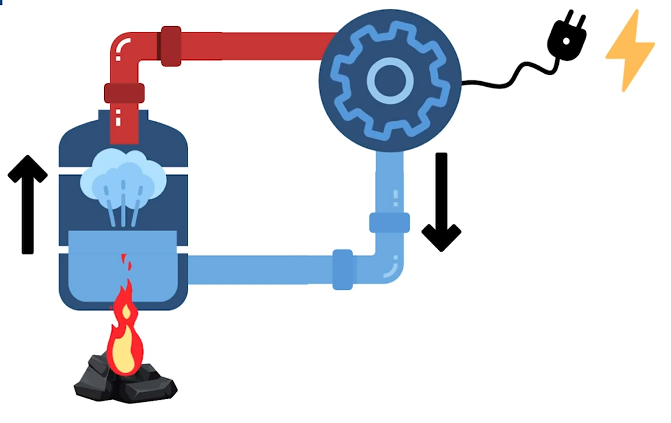
\includegraphics[width=0.7\linewidth]{../images/coal_based_electricity_production}
	\caption{Coal-based electricity production}
	\label{fig:coalbasedelectricityproduction}
\end{figure}

\ \\
Gas power plants, particularly modern combined cycles, exhibit higher efficiencies (55-60\%) by incorporating compressor-combustion chamber-turbine combinations and steam cycles. This flexibility is advantageous, allowing rapid adjustments in output power. The type of gas used in these processes, such as methane from rocky layers (shale gas) or methane originating from biological processes like fermentation, raises environmental considerations.\\
\\
The thermodynamic conversion of heat into electricity also includes nuclear reactions, either through fission or fusion. Nuclear fission involves splitting heavy elements like Uranium, producing heat for electricity generation. Despite its carbon-free nature, issues of radioactive waste disposal and limited fuel availability underscore its challenges. Commercial nuclear fission power plants are very big units producing 100s of MWs to more than a GW of power and are not very flexible in their output. Nuclear fusion, where light elements fuse to generate heat, remains under development, requiring extensive research for potential commercial viability.

\subsubsection{Renewable energy sources}

Efforts to enhance energy efficiency have led to the development of direct and weather-driven methods of electricity production, bypassing the thermodynamic losses associated with steam or gas-based cycles. One notable example is the use of photovoltaic (PV) cells, employing semiconductor technology to directly convert sunlight into electricity. These cells, arranged in modular panels on roofs, fields, and even floating structures on water, offer a renewable and carbon-emission-free source of electricity. However, their intermittent nature, limited to daylight hours, presents a challenge for continuous power generation.\\
\\
Wind power, another weather-driven source, harnesses the kinetic energy of wind to drive free-standing turbines with built-in generators. While wind farms on land are subject to weather fluctuations, offshore wind farms prove to be a more constant and predictable source of renewable electricity. Similar to PV production, the reliance on weather conditions remains a consideration.
\newpage
\ \\
Hydropower, based on the controlled release of water through turbine-generator combinations, offers another renewable and carbon-emission-free electricity production method. Operating on the principle of storing water in dams, this source is linked to river flow influenced by rainfall or melting snowpacks. However, the construction of large dams raises environmental concerns, causing landscape distortion, habitat destruction, and displacement of communities. These factors limit the expansion and designation of hydropower as a truly renewable source.

\subsubsection{Energy costs}

The costs associated with electricity production span two categories: capital investment for construction and operational expenses, including fuel, system costs, maintenance, and waste treatment. The affordability of energy sources varies, with some technologies exhibiting low initial construction costs but higher operational expenses, while others, like photovoltaic (PV) and wind-based generation, boast minimal ongoing costs post-construction. To facilitate a comprehensive comparison, the "levelized cost of electricity" (LCOE) serves as a valuable metric. LCOE enables the incorporation of all costs throughout an installation's lifetime, providing an averaged perspective per unit of electrical energy produced.\\
\\
The learning curve (figure \ref{fig:costofenergybytech}), where technologies tend to become cheaper as they mature, is a notable factor. However, nuclear energy appears to be an exception due to increased safety measures and waste treatment costs, rendering it relatively more expensive. Conversely, wind and PV energy have witnessed remarkable cost reductions, particularly with a tenfold drop in the price of PV over a decade. This dramatic shift is attributed to production upscaling, technological advancements, and maturation of these industries.

\begin{figure}[H]
	\centering
	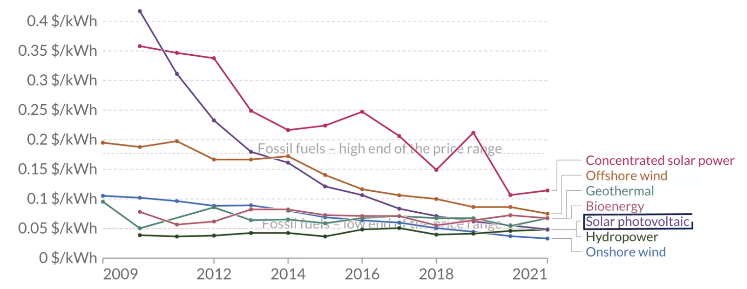
\includegraphics[width=0.8\linewidth]{../images/cost_of_energy_by_tech}
	\caption{Cost of energy by technology}
	\label{fig:costofenergybytech}
\end{figure}

\ \\
Despite their cost dynamics, wind and PV technologies have experienced significant growth in recent years. The system-level implications are crucial, considering the balance between energy production and consumption. In systems relying heavily on weather-related renewable sources, such as solar power, challenges emerge, especially during the transition between abundant sunlight during the day and nighttime.\\
\\
The "duck curve" (figure \ref{fig:duckcurve}) visually illustrates the need for alternative power sources during these transitions, which can include batteries, controlled power plants, or electricity grid exchanges with connected regions. Zooming out over a series of days introduces additional challenges, notably on cloudy days or those with reduced wind, often referred to as "Dunkelflaute" (a German term). A practical solution involves a diversified mix of generation technologies and international energy exchanges to ensure a reliable and balanced electricity supply.

\begin{figure}[H]
	\centering
	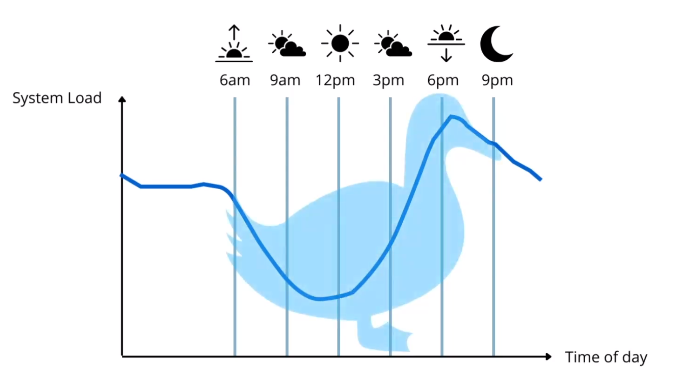
\includegraphics[width=0.7\linewidth]{../images/duck_curve}
	\caption{The duck curve}
	\label{fig:duckcurve}
\end{figure}

\subsection{Energy networks}

In our exploration of energy, it's essential to recognize the critical role played by distribution networks in transporting energy, particularly electricity, heat, and gas, from production sources to end consumers. These intricate networks operate across various geographical scales, spanning entire continents down to the confines of individual homes.\\
\\
Electricity grids, the most familiar to many, include transmission grids at the highest level, often recognized by high-voltage lines traversing landscapes. These lines can extend over considerable distances, sometimes hundreds of kilometers. The transmission grid incorporates large meshes connecting substations to enhance reliability. Additionally, underground cables, and even undersea cables, are utilized for more localized transmission, but cost much more unless you use so-called direct current electricity instead of alternating current electricity.\\
\\
Local distribution grids, found in most countries, operate at a more regional level with underground cables. Unlike the transmission grid, the distribution grid is radial in topology, employing multiple voltages. As the grid approaches individual homes, transformers step down the voltage to a safe level. Within homes, a miniature radial electricity grid continues, branching off from the main distribution system to power various appliances and systems.\\
\\
Similar to electricity networks, gas grids consist of cross-country transmission components and local distribution networks. Heat networks, on the other hand, are localized systems connecting heat sources, such as industrial waste heat, with nearby consumers. These networks play a crucial role in optimizing energy use and reducing waste.\\
\\
These days, it is almost impossible to run all those energy networks without digital tools for management or protection. Therefore, the presence of a dependable communication system is a necessity. In fact, the whole energy system is a so-called system of systems.

\begin{figure}[H]
	\centering
	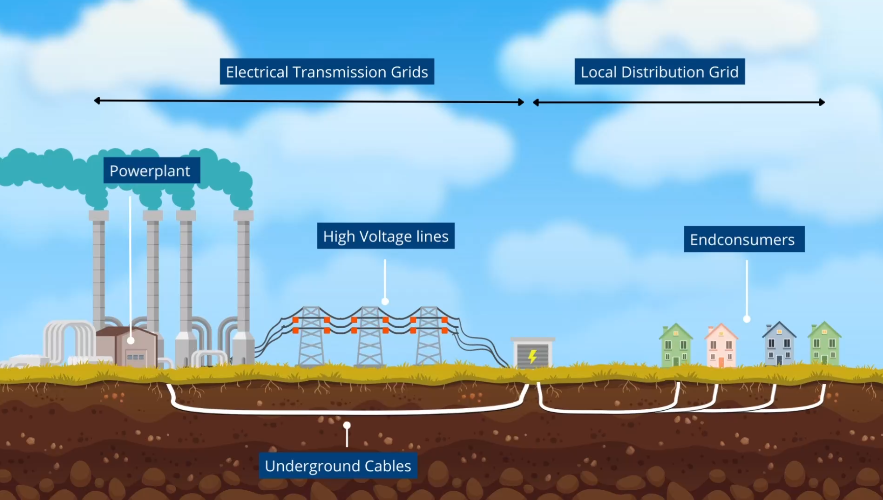
\includegraphics[width=0.8\linewidth]{../images/electricity_grid}
	\caption{The electricity grid}
	\label{fig:electricitygrid}
\end{figure}

\subsection{Energy use}
\subsubsection{Energy efficiency}

In analyzing energy consumption, it is crucial to examine where and how energy is utilized. In many European countries, roughly one-third of energy is consumed in industrial processes, another one-third is allocated to transportation, and the remaining portion is used in the built environment for services like heating and lighting. Conversion efficiency plays a pivotal role, emphasizing that the most cost-effective and sustainable kilowatt-hour of energy is the one that doesn't need to be produced. Encouraging consumers to maximize efficiency proves challenging, given their often limited awareness of energy quantities and the total cost of consumption.\\
\\
Efficiency considerations are evident in technological advancements, such as lighting. Historically, candles were used, but with Thomas Edison's introduction of electric light bulbs, efficiency was below 20\%, with 80\% of electricity turning into heat. Energy-saving lights in the late 20th century reduced energy consumption by about four times compared to traditional bulbs. Today, LED lights are 8 to 10 times more efficient and have a significantly longer lifespan. Convincing consumers to adopt such efficient technologies is challenging, especially when purchasing goods like washing machines, where considerations typically revolve around performance and price rather than energy consumption.\\
\\
Energy labels are often used to make consumers aware of a device's energy consumption, providing qualitative and quantitative information. Some regulators even prohibit certain technologies, like old-fashioned light bulbs. However, replacing an energy-consuming device with a more efficient one may not result in a proportional reduction in overall energy consumption due to rebound effects. Direct rebound involves users compensating for energy savings by using more of the efficient device, while indirect rebound sees savings spent on other energy-consuming goods. Additionally, pre-bound effects acknowledge that individuals with tight budgets may struggle to afford new energy-saving technologies, highlighting a socio-economic dimension to energy efficiency challenges.
\newpage
\ \\

\subsubsection{Energy consumption}

Examining your household energy consumption is crucial in understanding the broader energy landscape. In a Central European country like Belgium, households typically consume about 4 megawatt-hours of electricity annually, with heating demands using natural gas being 3 to 4 times higher. To lower these numbers and enhance sustainability, various measures can be taken.\\
\\
In the realm of building infrastructure, incorporating photovoltaic panels on roofs for local electricity production is a common approach. However, this may lead to challenges, such as overloading the electricity grid when excess solar electricity is produced simultaneously. Solutions include activating local energy demand and utilizing home batteries. Thermally insulating buildings and transitioning away from fossil fuels for heating, favouring heat pumps, are also advocated. Heat pumps, driven by electricity, significantly reduce energy needs (3 to 5 times less energy) and carbon dioxide emissions.\\
\\
The idea of replacing natural gas with hydrogen in the gas grid is considered, but efficiency concerns arise. The production of hydrogen through sustainable electrolysis involves multiple processes, leading to significant losses in efficiency compared to the direct electric route with heat pumps.\\
\\
Transportation, a significant energy consumer, has witnessed a shift towards electric vehicles. Battery electric cars, powered by modern batteries and electrical drives, emit at least three times fewer CO2 emissions than their fossil fuel counterparts. The electric car's silent operation also eliminates nitrous oxide and fine particle emissions. Despite previous beliefs in hydrogen-powered vehicles, the efficiency of battery electric cars remains superior.\\
\\
While direct electrification is advancing in various sectors, challenges persist in industries where chemical processes necessitate atomic building blocks sourced from fossil fuels. Finding circular solutions for carbon and efficient hydrogen production using electricity becomes imperative in these cases. The overall goal is to optimize energy consumption in various sectors through efficient technologies and sustainable practices.

\subsection{Energy storage}

In the transition to more sustainable technologies, the role of energy storage, particularly electricity storage, is significant. Examples include the electric car and home batteries. While batteries have been in existence for decades, the relatively recent emergence of lithium batteries is considered a key enabler of the energy transition. Mass production has drastically reduced the price of lithium batteries by a factor of 10 in the last decade.\\
\\
Lithium batteries offer several advantages. They can be charged and discharged hundreds or even thousands of times without a significant reduction in capacity. Additionally, they are compact and possess high energy and power density. Modern lithium batteries no longer contain toxic materials like cobalt and are fully recyclable. This progress addresses environmental concerns associated with older lithium battery types.\\
\\
Batteries are effective for balancing electricity production and demand over short terms, such as within a day or throughout a week. However, for balancing energy over more extended periods, such as between seasons, alternative forms of energy storage are required. Thermal storage and pumped hydro storage using large water basins are examples of technologies suitable for longer-term energy storage and play a crucial role in achieving a stable and sustainable energy grid.
\\\\

\subsection{Energy policies and markets}
\subsubsection{Energy markets}

The energy transition in Europe involves not just technological advancements but also significant economic shifts. The electricity and gas market has moved towards a "free" market system since the turn of the century, where energy prices are determined by supply and demand rather than fixed upfront. With the rise of renewable energy sources and increased stress on energy grids, electricity tariffs are now driven more by capital costs than operational costs, prompting a shift from kilowatt-hour-based to capacity-based charging. To benefit consumers, new business models supported by digital energy metering technologies are crucial, with plans to replace analogue meters with digital ones for all end consumers in the short term, though managing the resulting data poses a significant challenge.

\subsubsection{Energy policies}

The energy transition requires coordinated efforts from all policy makers and government levels, including European directives. The emission trading system (ETS) is an example of internationally coordinated policy measures, awarding tradeable rights to emit CO2 and setting goals to reduce emissions by the middle of the century. In this way the technologies that can mitigate CO2 emissions in the most economic way will be favoured. In practice this works like a carbon tax. This system is expected to expand into transportation and other fossil fuel usage.

\end{document}